\begin{frame}{L2 — the exchange profile}
	\begin{columns}[T]
		\begin{column}{0.55\textwidth}
			\centering
			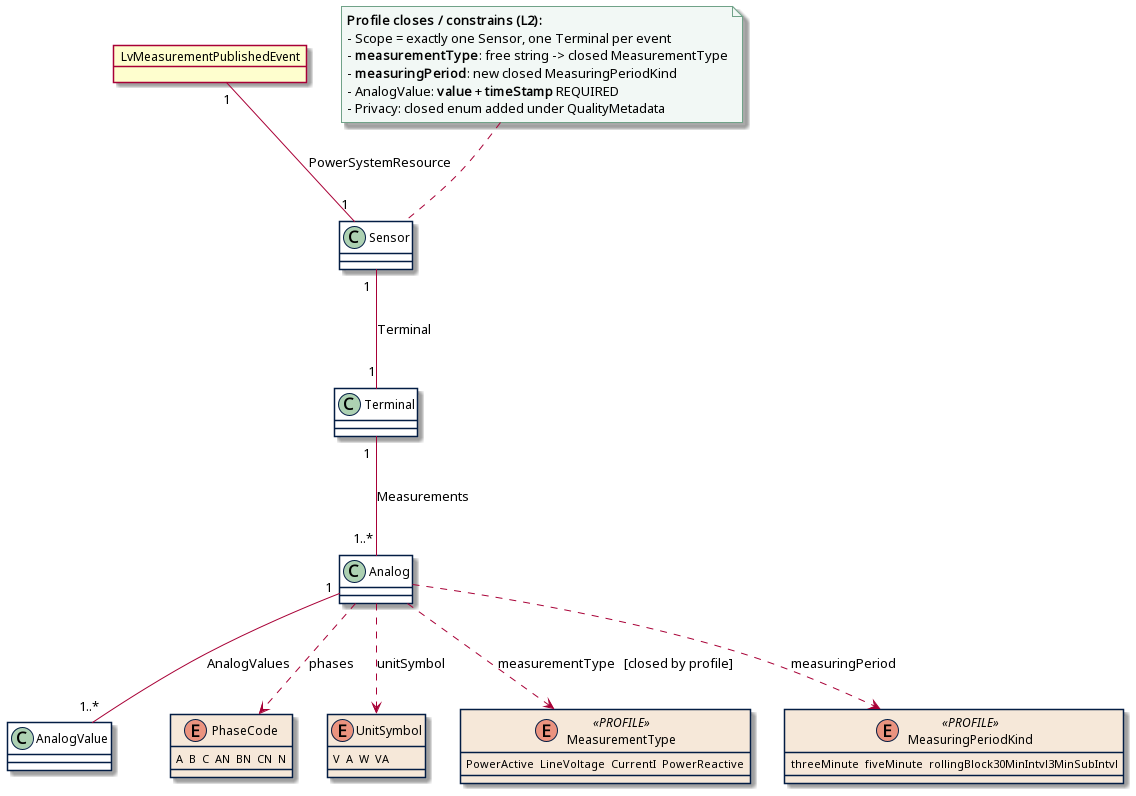
\includegraphics[width=\linewidth]{slides/profiles/example-profile/figs/profile.png}
		\end{column}
		\begin{column}{0.43\textwidth}
			\textbf{What the profile adds over the IM (constraints only):}
			\begin{itemize}
				\scriptsize
				\item two L1 enums \emph{closed} to the values of this exchange:
				  \texttt{MeasuringPeriodKind} and \texttt{Privacy}
				\item \texttt{measurementType} closed to: \texttt{PowerActive}, \texttt{LineVoltage}, \texttt{CurrentI}, \ldots
				\item required fields: every \texttt{AnalogValue} \emph{must} have \texttt{timeStamp} + \texttt{value}
				\item cardinalities: exactly one \texttt{Sensor}, one \texttt{Terminal} per event
			\end{itemize}
			\begin{block}{Still no format anywhere}
			\end{block}
		\end{column}
	\end{columns}
	\vspace{0.3em}
	This is the \emph{only} place those decisions are written down —
	not in three schema files, not in a wiki page.
\end{frame}
